\documentclass[
	12pt, 
	a4paper,
	numbers=noenddot, %Entfernt Punkt hinter Gliederungsnummern
	ngerman,
	headsepline, %Headertrennlinie
    oneside,
    version=first
	]{scrbook}

% ------- Imports ----------

\usepackage[T1]{fontenc}
\usepackage[utf8]{inputenc}
\usepackage[ngerman]{babel}
\usepackage{float}
\usepackage{url}
\usepackage{cite}
\usepackage{setspace}
\usepackage[acronym, nonumberlist]{glossaries}
\usepackage{listings,xcolor}
\usepackage[a4paper, margin=1in]{geometry}
\usepackage[normalem]{ulem}
\usepackage{graphicx}
\usepackage{chngcntr}
\usepackage{tgbonum}
\usepackage{subfig}
\usepackage{color, colortbl}

\usepackage{metadata}
\usepackage{lib/customcommands}

\usepackage[ 
   colorlinks,        % Links ohne Umrandungen in zu wählender Farbe 
   linkcolor=black,   % Farbe interner Verweise 
   filecolor=black,   % Farbe externer Verweise 
   citecolor=black,   % Farbe von Zitaten 
   urlcolor=blue	  % Farbe von Links
]{hyperref}

% --------Settings----------

% falsche Default-Silbentrennung überschreiben
% \hyphenation{Soft-ware-ent-wick-lung}
\geometry{verbose,tmargin=3cm,bmargin=2cm,lmargin=3cm,rmargin=3cm} 
\renewcommand*{\glspostdescription}{}

\setlength{\footskip}{10mm}

\counterwithout{figure}{chapter}
\counterwithout{table}{chapter}

\definecolor{dkgreen}{rgb}{0,.6,0}
\definecolor{dkblue}{rgb}{0,0,.6}
\definecolor{dkyellow}{cmyk}{0,0,.8,.3}

\definecolor{zcgray}{rgb}{.7, .7, .7}

\clubpenalty = 10000 \widowpenalty = 10000 \displaywidowpenalty = 10000
\addtokomafont{caption}{\small} 

\addto\extrasngerman{
    \def\sectionautorefname{Kapitel}
    \def\subsectionautorefname{Kapitel}
    \def\subsubsectionautorefname{Kapitel}
}

\lstset{
    numbers=left, 
    numberstyle=\tiny, 
    numbersep=5pt,
    breaklines=true,
    frame=single,
    language=sh,
    basicstyle=\ttfamily\fontsize{10}{12}\selectfont,
    keywordstyle    = \color{dkblue},
    stringstyle     = \color{red},
    identifierstyle = \color{dkgreen},
    commentstyle    = \color{gray},
    emph            =[1]{php},
    emphstyle       =[1]\color{black},
    emph            =[2]{if,and,or,else},
    emphstyle       =[2]\color{dkyellow}
}

\renewcommand*{\glspostdescription}{}

% sorgt dafür, dass bei Leerzeile die Einrückung verhindert und stattdessen eine Leerzeile eingefügt wird % erspart bigskips und erhöht die Lesbarkeit im LaTeX-Text 
\KOMAoptions{parskip=full*}

% ändert Titelschriftart in Serifen-Normalschriftart
\addtokomafont{disposition}{\rmfamily} 

\makenoidxglossaries{}
\loadglsentries{misc/glossary.tex}

% \fontfamily{Arial}\selectfont
\sloppy

% --------Environments------

\newenvironment{reqtable}{
	\begin{tabular}{| p{0.05\linewidth} | p{0.35\linewidth} | p{0.5\linewidth} |}
        \hline
        \rowcolor{zcgray}
	\textbf{Nr.} & \textbf{Anforderung} & \textbf{Erläuterung}\\ \hline
}{
	\hline
	\end{tabular}
}

% --------Title------------

\begin{document}
\begin{titlepage}
	\begin{figure*}[ht!]
		
\includegraphics[width=0.45\textwidth]{img/th_header_logo.png} \hfill
		
\includegraphics[width=0.45\textwidth]{img/hwr_header_logo.png}
	\end{figure*}
	\vspace{20pt}
	\centering \textbf{\huge \zTyp}
	\normalfont\endgraf\rule{\textwidth}{.4pt}\endgraf{}
	\begingroup
		\centering
		\linespread{2.5}
		\huge\zTitel{}
	\endgroup
	\linespread{1.5}
	\endgraf\rule{\textwidth}{.4pt}
	\hfill
	\begin{center}
		\textbf{\today}
		\endgraf{}
	\end{center}
	\begin{tabular}{rl}
		\textbf{\normalsize{Name, Vorname:}}        & \normalsize{\zStudent} \\
		\textbf{\normalsize{Matrikelnummer:}}       & \normalsize{\zMatrikelnr} \\
		\textbf{\normalsize{Ausbildungsbetrieb:}}   & \normalsize{\zBetrieb} \\
		\textbf{\normalsize{Studienjahrgang:}}      & \normalsize{\zJahrgang} \\
		\textbf{\normalsize{Fachbereich:}}          & \normalsize{\zFachbereich} \\
		\textbf{\normalsize{Studiengang:}}          & \normalsize{\zStudiengang} \\
		\textbf{\normalsize{Modul:}}                & \normalsize{\zModul} \\
		\textbf{\normalsize{Betreuer Hochschule:}}  & \normalsize{\zBetreuerHs} \\
		\textbf{\normalsize{Betreuer Unternehmen:}} & \normalsize{\zBetreuerUn} \\
		\textbf{\normalsize{Anzahl der Wörter}}     & \normalsize{\zAnzahlWoerter} \\
	\end{tabular}
	\endgraf{}
	\vspace{50pt}
	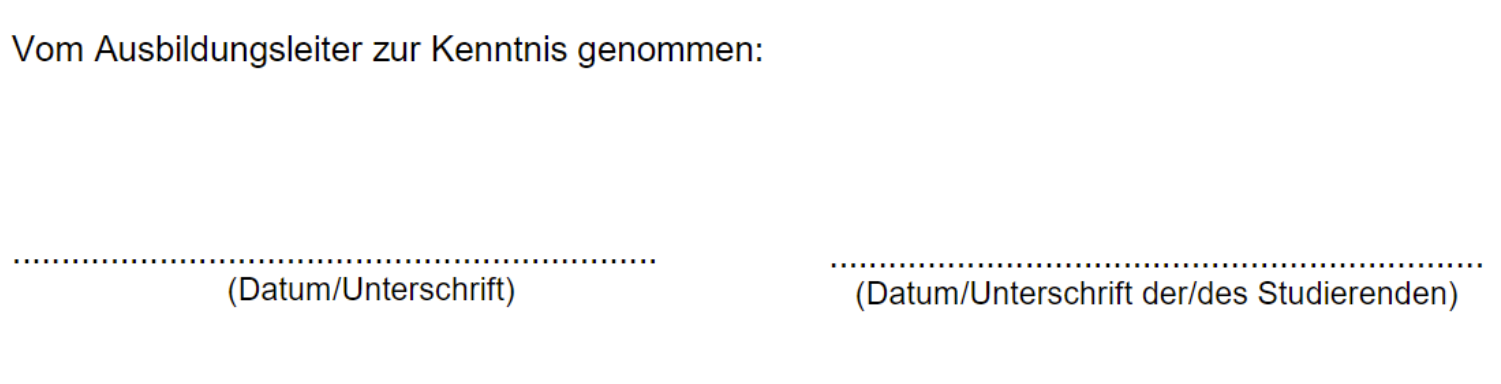
\includegraphics[scale=0.5]{img/ptb-signature.png}
\end{titlepage}

% --------Abstract----------

\chapter*{Abstract}

\addcontentsline{toc}{chapter}{Abstract}


%--------------------------

\pagenumbering{Roman}
\newpage
\newpage


\tableofcontents{}
\addcontentsline{toc}{chapter}{Inhaltsverzeichnis}

%\listoffigures
%\addcontentsline{toc}{chapter}{Abbildungsverzeichnis}
%\listoftables
%\addcontentsline{toc}{chapter}{Tabellenverzeichnis}

\printnoidxglossaries{}
\addcontentsline{toc}{chapter}{Akronyme}

\clearpage

%% arabische Seitenzahlen
\pagenumbering{arabic}

% --------Content----------

% \include{chapters/chaptername}

% -------------------------

\bibliography{./misc/bibliography}
\bibliographystyle{./lib/hwrbib}
\addcontentsline{toc}{chapter}{Literaturverzeichnis}

% -Ehrenwörtliche Erklärung-

\chapter*{Ehrenwörtliche Erklärung}

\addcontentsline{toc}{chapter}{Ehrenwörtliche Erklärung}

\thispagestyle{empty}

Ich erkläre ehrenwörtlich:
\begin{enumerate}
	\item dass ich meinen Praxistransferbericht selbstständig verfasst habe,
	\item dass ich die Übernahme wörtlicher Zitate aus der Literatur sowie die Verwendung der Gedanken anderer Autoren an den entsprechenden Stellen innerhalb der Arbeit gekennzeichnet habe,
	\item dass ich meinen Praxistransferbericht bei keiner anderen Prüfung vorgelegt habe.
\end{enumerate}
Ich bin mir bewusst, dass eine falsche Erklärung rechtliche Folgen haben wird.

\vspace{2cm}

\begin{tabular}{lp{4em}l}
	\hspace{5cm} &  & \hspace{4cm} \\\cline{1-1}\cline{3-3}
	Ort, Datum   &  & \zStudent
\end{tabular}

%--------------------------

\end{document}